\documentclass[twoside]{article}

\input{../common/preamble}
\input{../common/preamble-zh}
\newcommand{\Hom}{\operatorname{Hom}}
\newcommand{\Sp}{\mathbf{sp}}
\newcommand{\colim}{\mathrm{colim}}
\newcommand{\im}{\operatorname{im}}
\newcommand{\vp}{\varphi}
\newcommand{\supp}{\mathrm{supp}}
\newcommand{\tr}{\operatorname{tr}}
\newcommand{\YP}{]Y[_\CP}
\newcommand{\XP}{]X[_\CP}
\newcommand{\ZP}{]Z[_\CP}
\newcommand{\HSn}{H^n_{cris}(X/S)}
\newcommand{\Hkn}{H^n_{cris}(X/W(k))}
\newcommand{\HSd}{H^\cdot_{cris}(X/S)}
\newcommand{\Hkd}{H^\cdot_{cris}(X/W(k))}
\newcommand{\HCd}{H^\cdot_{conv}(X)}
\newcommand{\HCn}{H^n_{conv}(X)}
\newcommand{\HRd}{H^\cdot_{rig}(X)}
\newcommand{\HRn}{H^n_{rig}(X)}
\newcommand{\DRX}{\Omega_{\XP/K}^\cdot}
\newcommand{\DRY}{\Omega_{\YP/K}^\cdot}
\newcommand{\Spec}{\mathrm{Spec}}
\newcommand{\Spf}{\mathrm{Spf}}
\newcommand{\Spp}{\mathrm{Sp}}
\newcommand{\Frac}{\mathrm{Frac}}
\newcommand{\DRXn}{\Omega_{\XP/K}^n}
\newcommand{\BA}{{\mathbb {A}}}
\newcommand{\BB}{{\mathbb {B}}}
\newcommand{\BC}{{\mathbb {C}}} 
\newcommand{\BD}{{\mathbb {D}}}
\newcommand{\BE}{{\mathbb {E}}} 
\newcommand{\BF}{{\mathbb {F}}}
\newcommand{\BG}{{\mathbb {G}}} 
\newcommand{\BH}{{\mathbb {H}}}
\newcommand{\BI}{{\mathbb {I}}} 
\newcommand{\BJ}{{\mathbb {J}}}
\newcommand{\BK}{{\mathbb {K}}} 
\newcommand{\BL}{{\mathbb {L}}}
\newcommand{\BM}{{\mathbb {M}}} 
\newcommand{\BN}{{\mathbb {N}}}
\newcommand{\BO}{{\mathbb {O}}} 
\newcommand{\BP}{{\mathbb {P}}}
\newcommand{\BQ}{{\mathbb {Q}}} 
\newcommand{\BR}{{\mathbb {R}}}
\newcommand{\BS}{{\mathbb {S}}} 
\newcommand{\BT}{{\mathbb {T}}}
\newcommand{\BU}{{\mathbb {U}}} 
\newcommand{\BV}{{\mathbb {V}}}
\newcommand{\BW}{{\mathbb {W}}} 
\newcommand{\BX}{{\mathbb {X}}}
\newcommand{\BY}{{\mathbb {Y}}} 
\newcommand{\BZ}{{\mathbb {Z}}}
\newcommand{\CA}{{\mathcal {A}}} 
\newcommand{\CB}{{\mathcal {B}}}
\newcommand{\CC}{{\mathcal {C}}} 
\newcommand{\CD}{{\mathcal {D}}}
\newcommand{\CE}{{\mathcal {E}}} 
\newcommand{\CF}{{\mathcal {F}}}
\newcommand{\CG}{{\mathcal {G}}} 
\newcommand{\CH}{{\mathcal {H}}}
\newcommand{\CI}{{\mathcal {I}}} 
\newcommand{\CJ}{{\mathcal {J}}}
\newcommand{\CK}{{\mathcal {K}}} 
\newcommand{\CL}{{\mathcal {L}}}
\newcommand{\CM}{{\mathcal {M}}} 
\newcommand{\CN}{{\mathcal {N}}}
\newcommand{\CO}{{\mathcal {O}}} 
\newcommand{\CP}{{\mathcal {P}}}
\newcommand{\CQ}{{\mathcal {Q}}} 
\newcommand{\CR}{{\mathcal {R}}}
\newcommand{\CS}{{\mathcal {S}}} 
\newcommand{\CT}{{\mathcal {T}}}
\newcommand{\CU}{{\mathcal {U}}} 
\newcommand{\CV}{{\mathcal {V}}}
\newcommand{\CW}{{\mathcal {W}}} 
\newcommand{\CX}{{\mathcal {X}}}
\newcommand{\CY}{{\mathcal {Y}}} 
\newcommand{\CZ}{{\mathcal {Z}}}

\addbibresource{ASM.bib}
\nocite{*}

\begin{document}

\title{变号矩阵与可积系统\\\large{——从一道新领军测试题到现代数学}}
\author{徐凯\footnote{原清华大学数学系数 41 班.}}
\headertitle{变号矩阵与可积系统}

\begin{abstract}
    在这篇短文中,
    我们从变号矩阵的计数问题出发,
    将其表述为六顶点模型中态和的计算,
    并通过 Yang--Baxter 方程和可积性给出问题的显式解.
\end{abstract}

清华大学2021年新领军综合测试中有如下一道试题: 

\begin{problem}
    要求矩阵满足条件:  (1) 只有三种元素$-1,0,1$;  (2) 每一行每一列不全为0;  (3) 每行每列在去掉所有 $0$ 之后, 剩下的元素均形如 $1,-1,1,\dotsc,-1,1$. 已知这样的三阶矩阵有7个, 求四阶的有多少. 
\end{problem}

这道题目虽然表述完全初等, 但背后蕴藏非常丰富的结构, 是中学阶段的同学接触现代数学之深邃高明十分难得的机会, 故撰此文聊作剖析, 以为引玉之砖. 本文主要证明来自G.Kuperberg. 


\section{变号矩阵到六顶点模型}
我们首先重新表述变号矩阵的计数问题,将其化归为统计力学中的六顶点模型. 

在六顶点模型中, 我们关心平面上每边带定向, 并且每个顶点恰好有两条边进入两条边离开的正方形图, 每一个这样的图称为一个态(state). 给定一个态, 在每个顶点附近有如下六种可能的定向: 
\[
    \sixvertex{$a$}{$b$}{$c$}{$d$}{$e$}{$f$}
\]

我们为每一种可能$i$赋一个权重$w(i)$, 每个顶点的权重相乘定义为图的权重, 而 (满足给定条件的) 所有态的权重之和称为态和(state sum). 六顶点模型中也可设置边界条件, 即引入只连一条 (给定) 定向边的顶点. 特别的, 我们可以考虑$n\times n$方形网格, 再加左右两侧向内上下两侧向外的边界条件, 这个模型称为方冰 (square ice). 一个方冰态可以用如下对应转化为一个变号矩阵: (注意这里的$-1,0,1$和权重无关)
$$
\sixvertex{$1$}{$-1$}{$0$}{$0$}{$0$}{$0$}
$$
并且可以验证这是一个一一对应. 因此, 变号矩阵的计数问题即等价于六顶点模型所有权重为1的态和. 故我们只需求解六顶点模型即可. 六顶点模型可以严格求解, 其中的核心结构为Yang--Baxter方程 (以下简称YBE). 

\section{YBE的场论来源}
这一节中我们简短介绍YBE在场论中的起源. 可积场论可以视为可积格点模型 (lattice model) 的连续极限. 譬如六顶点模型取时间方向的连续极限得到Heisenberg自旋链(spin chain), 时空均取连续极限得到正弦Gordon模型, 正弦Gordon模型即为最简单的可积场论之一. 本节内容与后文内容并无逻辑关联, 仅通过一个自然的来源以启发YBE这一概念, 故相对简略, 不感兴趣的读者可以跳过本节. 

 (相对论场论中) 可积性是一个仅存在于二维的独特现象, 事实上, Coleman--Mandula论证了在更高维度, 倘若存在自旋至少为2的守恒荷, 则我们总可以利用相应的对称性移动粒子到一般位置, 使得他们的轨迹永不相交, 不会发生散射因而$S$矩阵(即粒子散射过程中初始状态到最终状态的线性变换)一定为$1$.

但平面上两条一般位置的直线总会相交, 故以上论证不能成立. 然而我们总能通过移动至一般位置避免三条直线交于一点, 这时所有散射都为两两弹性碰撞, 所以全部散射振幅都由弹性碰撞的所决定. 另外, 给定三条定向直线$l,m,n$, 倘若$m,n$交点在$l$左侧, 那么我们总是可以利用前文的对称性将其移动到右侧. 这时得到的构型与先前并不拓扑等价, 二者散射振幅相等需要弹性碰撞的散射振幅满足一个三次方程, 即为YBE (这时动量是其中的一个谱参数). 

\section{六顶点模型的解}
取一个未定元$q$, 记$[x]=\frac{q^{x/2}-q^{-x/2}}{q^{1/2}-q^{-1/2}}$, 对一个带$x$标记的顶点
\[
    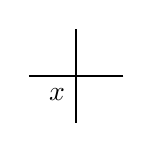
\begin{tikzpicture}[
        scale = .6,
        thick
    ]
        \begin{scope}[shift={(0,0)}]
            \draw (-1, 0)--( 0, 0);
            \draw ( 1, 0)--( 0, 0);
            \draw ( 0, 0)--( 0, 1);
            \draw ( 0, 0)--( 0,-1);
            \node at (-.4, -.4) {$x$};
        \end{scope}
    \end{tikzpicture}    
\]
我们为六种定向赋权如下: 
$$
\sixvertex{$-q^{-x/2}$}{$-q^{x/2}$}{$[x-1]$}{$[x-1]$}{$[x]$}{$[x]$}
$$

这可以视为指定了一个二维场论的弹性碰撞(大小为$2^2\times 2^2$的) $S$矩阵(在可积格点模型中通常称为$R$矩阵), 而YBE正是这个可积场论的相容性条件: 
\begin{theorem}[Baxter]  若 $x
= y + z$,  则 $R$-矩阵 $R(x)$, $R(y)$, 和 $R(z)$ 满足如下两图对应矩阵相等
\[
    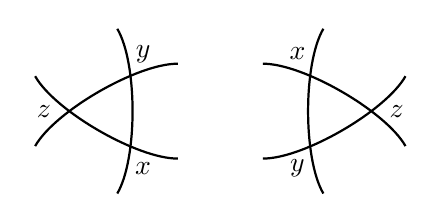
\begin{tikzpicture}[
        scale = .7,
        thick
    ]
        \begin{scope}[shift={(0,0)}]
            \draw (-85:1.5) .. controls (-60:1) and (60:1) .. (85:1.5);
            \draw (35:1.5) .. controls (60:1) and (180:1) .. (205:1.5);
            \draw (155:1.5) .. controls (180:1) and (-60:1) .. (-35:1.5);
            \node at (-60:1.2) {$x$};
            \node at (60:1.2) {$y$};
            \node at (180:1.2) {$z$};
        \end{scope}
        \begin{scope}[shift={(4,0)}]
            \draw (95:1.5) .. controls (120:1) and (-120:1) .. (-95:1.5);
            \draw (-145:1.5) .. controls (-120:1) and (0:1) .. (25:1.5);
            \draw (-25:1.5) .. controls (0:1) and (120:1) .. (145:1.5);
            \node at (120:1.2) {$x$};
            \node at (-120:1.2) {$y$};
            \node at (0:1.2) {$z$};
        \end{scope}
    \end{tikzpicture}    
\]
\end{theorem}
我们首先解释何为两图对应的矩阵: 一言以蔽之, 他们是这个散射图对应的$S$矩阵. 每个图都有六条外边, 并有自然的一一对应. 他们共有64种定向, 每种定向都可以作为边界条件得到一个态和, 这正是这些矩阵的项. 

我们将权重的定义延拓到更一般的光滑曲线系统上.
对一种选定的定向方式,
约定每个切线水平向左的点, 若上凸则赋权$-q^{1/2}$,下凸则$-q^{-1/2}$,
切线水平向右的点则赋权$1$,
然后乘起来得到一个单项式.
把每种定向方式所得到的单项式加起来, 得到的多项式就是态和.
我们有如下的态和表达式:
\[
    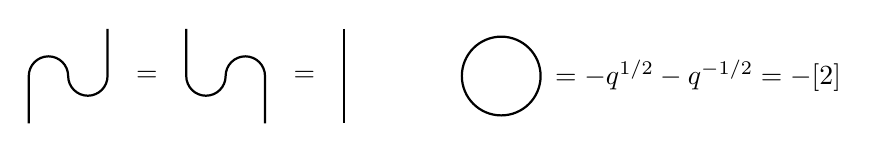
\begin{tikzpicture}[
        scale = .5,
        thick
    ]
        \begin{scope}[shift={(0,0)}]
            \draw (-1, -1.2) -- (-1, 0) arc (180:0:.5) arc (180:360:.5) -- (1, 1.2);
        \end{scope}
        \node at (2, 0) {$=$};
        \begin{scope}[shift={(4,0)}]
            \draw (-1, 1.2) -- (-1, 0) arc (180:360:.5) arc (180:0:.5) -- (1, -1.2);
        \end{scope}
        \node at (6, 0) {$=$};
        \draw (7, 1.2) -- (7, -1.2);

        \draw (11, 0) circle (1);
        \node[inner sep = 0] at (16, 0) {$= -q^{1/2} - q^{-1/2} = -[2]$};
    \end{tikzpicture}  
\]
% \begin{equation}
% \pspicture(-1,0)(1,1)
% \qline(-.7,-1)(-.7,0)
% \psarc(-.35,0){.35}{0}{180}\psarc(.35,0){.35}{180}{0}
% \qline(.7,0)(.7,1)
% \endpspicture
% =
% \pspicture(-1.2,0)(1.2,1)
% \qline(.7,-1)(.7,0)
% \psarc(.35,0){.35}{0}{180}\psarc(-.35,0){.35}{180}{0}
% \qline(-.7,0)(-.7,1)
% \endpspicture
% =
% \pspicture(-.5,0)(.5,.7)
% \qline(0,-.7)(0,.7)
% \endpspicture
% \hspace{2cm}
% \pspicture(-.7,0)(.7,.5)
% \pscircle(0,0){.5}
% \endpspicture
% = -q^{1/2} - q^{-1/2} = -[2]
% \label{etl}
% \end{equation}
% \\
可以看出曲线的贡献只取决于它的同伦类, 并且$R(x)$可以表示为
\[
    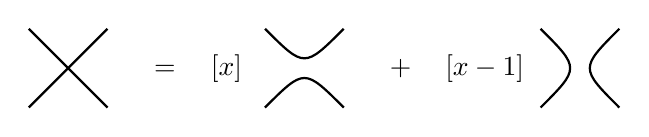
\begin{tikzpicture}[
        scale = .5,
        thick
    ]
        \begin{scope}[shift={(0,0)}]
            \draw (-1, -1) -- (1, 1) (-1, 1) -- (1, -1);
        \end{scope}
        \node at (3.3, 0) {$= \quad [x]$};
        \begin{scope}[shift={(6,0)}]
            \draw (-1, 1) .. controls (0, 0) and (0, 0) .. (1, 1);
            \draw (-1, -1) .. controls (0, 0) and (0, 0) .. (1, -1);
        \end{scope}
        \node at (9.8, 0) {${} + \quad [x - 1]$};
        \begin{scope}[shift={(13,0)}]
            \draw (-1, 1) .. controls (0, 0) and (0, 0) .. (-1, -1);
            \draw (1, 1) .. controls (0, 0) and (0, 0) .. (1, -1);
        \end{scope}
    \end{tikzpicture}  
\]
% \\
% $$
% \pspicture(-.7,-0.3)(.7,.7)
% \psline(.7;45)(.7;225)\psline(.7;135)(.7;315)
% \rput[t](0,-.2828){$x$}\endpspicture
% = 
% [x]
% \pspicture(-.9,-0.3)(.9,.7)
% \pccurve[angleA= 45,angleB=135,ncurv=1,nodesep=0](.7;225)(.7;315)
% \pccurve[angleA=225,angleB=315,ncurv=1,nodesep=0](.7; 45)(.7;135)
% \endpspicture
% +[x-1]
% \pspicture(-.9,-0.3)(.9,.7)
% \pccurve[angleA=225,angleB=135,ncurv=1,nodesep=0](.7; 45)(.7;315)
% \pccurve[angleA= 45,angleB=315,ncurv=1,nodesep=0](.7;225)(.7;135)
% \endpspicture
% $$

因此一个态和可以表示为对曲线的求和, 其中每个闭圈贡献一个因子 $-[2]$ (这种计算规则起源于Temperley--Lieb范畴, 与 $\mathfrak{sl}_2$的量子群密切相关). 由此直接计算便可验证YBE. 
以下我们记
\[
    \begin{tikzpicture}[
        scale = .6,
        thick
    ]
        \begin{scope}[shift={(0,0)}]
            \draw (-1, 0)--( 0, 0);
            \draw ( 1, 0)--( 0, 0);
            \draw ( 0, 0)--( 0, 1);
            \draw ( 0, 0)--( 0,-1);
            \node at (-1.4, 0) {$x$};
            \node at (0, -1.4) {$y$};
        \end{scope}
        \node at (2, 0) {$=$};
        \begin{scope}[shift={(4,0)}]
            \draw (-1, 0)--( 0, 0);
            \draw ( 1, 0)--( 0, 0);
            \draw ( 0, 0)--( 0, 1);
            \draw ( 0, 0)--( 0,-1);
            \node at (-.8, -.4) {$x - y$};
        \end{scope}
    \end{tikzpicture}    
\]
% $$
% \pspicture(-.9,0)(.9,.9)
% \psline(0,0)(0,.7)    \psline(0,0)(.7,0)
% \psline(-0,0)(-.7,0)  \psline(0,-0)(0,-.7)
% \rput[r](-.9,0){$x$}
% \rput[t](0,-.9){$y$}
% \endpspicture
% =
% \pspicture(-1.6,0)(.7,.9)
% \psline(0,0)(0,.7)    \psline(0,0)(.7,0)
% \psline(-0,0)(-.7,0)  \psline(0,-0)(0,-.7)
% \rput[rt](-.2,-.2){$x-y$}
% \endpspicture
% $$

对于$X=(x_i)$, $Y=(y_i)$, 记$Z(n,X,Y)$为如下的态和
\[
    \begin{tikzpicture}[
        scale = .8,
        thick,
        decoration={
            markings,
            mark=at position 0.65 with {\arrow{stealth}}
        }
    ]
        \draw[postaction={decorate}] (-1, 0)--( 0, 0);
        \draw[postaction={decorate}] (-1,-1)--( 0,-1);
        \draw[postaction={decorate}] (-1,-3)--( 0,-3);
        \draw[postaction={decorate}] ( 4, 0)--( 3, 0);
        \draw[postaction={decorate}] ( 4,-1)--( 3,-1);
        \draw[postaction={decorate}] ( 4,-3)--( 3,-3);
        \draw[postaction={decorate}] ( 0, 0)--( 0, 1);
        \draw[postaction={decorate}] ( 1, 0)--( 1, 1);
        \draw[postaction={decorate}] ( 3, 0)--( 3, 1);
        \draw[postaction={decorate}] ( 0,-3)--( 0,-4);
        \draw[postaction={decorate}] ( 1,-3)--( 1,-4);
        \draw[postaction={decorate}] ( 3,-3)--( 3,-4);
        \draw (0, 0) -- (0,-1.5) (0,-2.5) -- (0,-3);
        \draw (1, 0) -- (1,-1.5) (1,-2.5) -- (1,-3);
        \draw (3, 0) -- (3,-1.5) (3,-2.5) -- (3,-3);
        \draw (0, 0) -- (1.5, 0) (2.5, 0) -- (3, 0);
        \draw (0,-1) -- (1.5,-1) (2.5,-1) -- (3,-1);
        \draw (0,-3) -- (1.5,-3) (2.5,-3) -- (3,-3);
        \node at ( 2,-.5) {$\cdots$};
        \node at ( 2, -3) {$\cdots$};
        \node at (.5, -2) {$\vdots$};
        \node at ( 3, -2) {$\vdots$};
        \node at ( 2, -2) {$\ddots$};
        \node at (0, -4.4) {$y_0$};
        \node at (1, -4.4) {$y_1$};
        \node at (3, -4.4) {$y_{n-1}$};
        \node at (-1.4, 0) {$x_0$};
        \node at (-1.4,-1) {$x_1$};
        \node at (-1.6,-3) {$x_{n-1}$};
    \end{tikzpicture}
\]

% $$
% \pspicture(-1.5,-1.5)(4,4)
% \pnode(-1, 4){aa}\pnode(0, 4){ab}\pnode(1, 4){ac}\pnode(1.5, 4){ad}
% \pnode(2.5, 4){ax}\pnode(3, 4){ay}\pnode(4, 4){az}
% \pnode(-1, 3){ba}\pnode(0, 3){bb}\pnode(1, 3){bc}\pnode(1.5, 3){bd}
% \pnode(2.5, 3){bx}\pnode(3, 3){by}\pnode(4, 3){bz}
% \pnode(-1, 2){ca}\pnode(0, 2){cb}\pnode(1, 2){cc}\pnode(1.5, 2){cd}
% \pnode(2.5, 2){cx}\pnode(3, 2){cy}\pnode(4, 2){cz}
% \pnode(-1,1.5){da}\pnode(0,1.5){db}\pnode(1,1.5){dc}\pnode(1.5,1.5){dd}
% \pnode(2.5,1.5){dx}\pnode(3,1.5){dy}\pnode(4,1.5){dz}
% \pnode(-1,.5){xa}\pnode(0,.5){xb}\pnode(1,.5){xc}\pnode(1.5,.5){xd}
% \pnode(2.5,.5){xx}\pnode(3,.5){xy}\pnode(4,.5){xz}
% \pnode(-1, 0){ya}\pnode(0, 0){yb}\pnode(1, 0){yc}\pnode(1.5, 0){yd}
% \pnode(2.5, 0){yx}\pnode(3, 0){yy}\pnode(4, 0){yz}
% \pnode(-1,-1){za}\pnode(0,-1){zb}\pnode(1,-1){zc}\pnode(1.5,-1){zd}
% \pnode(2.5,-1){zx}\pnode(3,-1){zy}\pnode(4,-1){zz}
% \ncline[nodesepA=.2]{ba}{bb}\mto \ncline{bb}{bc}\ncline{bc}{bd}
% \ncline{bx}{by}\ncline[nodesepB=.2]{by}{bz}\mfro
% \ncline[nodesepA=.2]{ca}{cb}\mto \ncline{cb}{cc}\ncline{cc}{cd}
% \ncline{cx}{cy}\ncline[nodesepB=.2]{cy}{cz}\mfro
% \ncline[nodesepA=.2]{ya}{yb}\mto \ncline{yb}{yc}\ncline{yc}{yd}
% \ncline{yx}{yy}\ncline[nodesepB=.2]{yy}{yz}\mfro
% \ncline[nodesepA=.2]{ab}{bb}\mfro\ncline{bb}{cb}\ncline{cb}{db}
% \ncline{xb}{yb}\ncline[nodesepB=.2]{yb}{zb}\mto 
% \ncline[nodesepA=.2]{ac}{bc}\mfro\ncline{bc}{cc}\ncline{cc}{dc}
% \ncline{xc}{yc}\ncline[nodesepB=.2]{yc}{zc}\mto 
% \ncline[nodesepA=.2]{ay}{by}\mfro\ncline{by}{cy}\ncline{cy}{dy}
% \ncline{xy}{yy}\ncline[nodesepB=.2]{yy}{zy}\mto 
% \rput[r](ba){$x_0$}\rput[r](ca){$x_1$}\rput[r](ya){$x_{n-1}$}
% \rput[t](zb){$y_0$}\rput[t](zc){$y_1$}\rput[t](zy){$y_{n-1}$}
% \rput(.5,1){$\vdots$}\rput(2,1){$\ddots$}\rput(2,2.5){$\cdots$}
% \rput(2,0){$\cdots$}\rput(3,1){$\vdots$}
% \endpspicture
% $$

$Z$关于$x_i$和$y_i$分别都是对称的: 这可以由YBE直接证明, 也可以用第二节中YBE的场论推导类似可得. 这对$Z$的结构施加了很强的限制, 通过仔细分析它的零点与极点, 我们可以显式解得
\begin{theorem}[Izergin, Korepin] 
    \label{thkorepin}
    态和 $Z(n;X,Y)$ 有如下表达
    $$Z(n;X,Y) = {(-1)^n\left(\prod_{i=0}^{n-1} q^{(y_i-x_i)/2}\right)
    \prod_{0 \le i,j < n} [x_i-y_j][x_i-y_j-1] \over \left(\prod_{0 \le j<i<n}
    [x_i-x_j]\right)\left(\prod_{0 \le i < j < n} [y_i-y_j]\right)}\det M,$$
    其中
    $$M_{i,j} = {1 \over [x_i - y_j][x_i - y_j - 1]}.$$
\end{theorem}

由第一节的论证我们知道$n\times n$变号矩阵的数量恰好为方冰态数量, 而方冰态中顶点$a$ 比$b$多$n$个, $c,d$数目相等, $e,f$也相等, 所以可得变号矩阵数目为
$$ \biggl(\frac12\biggr)^{n-n^2}(-1)^n q^{n/4} Z_{1/2}(n)|_{x=1},$$
其中$Z_{1/2}(n)=Z(n;1/2,...,1/2,0,...,0)$. 


这是定理2中表达式的 (可去) 奇点, 使用L'H\^opital法则我们可以直接计算得如下表达式(计算细节请参见\cite{10.1155/S1073792896000128}): 
\begin{theorem}
$n\times n$变号矩阵数目为
\[ \frac{1! \, 4! \, 7! \cdots (3n-2)!}{n! \, (n+1)! \, (n+2)! \cdots (2n-1)!}. \]
\end{theorem}
由此我们就解决了变号矩阵的计数问题. 

\section{总结}
可积系统对现代数学的深刻影响远不止于此: YBE的解通常称为$R$矩阵, 是量子群与辫张量范畴的核心信息, 对其与场论的关系的研究启发了大量重要的数学. 譬如著名的Kazhdan--Lusztig等价联系起量子群的$R$矩阵与共形场论中Knizhnik--Zamolodchikov方程解的单性(monodromy). 又如Maulik--Okounkov通过$R$矩阵构造了瞬子模空间上同调上的量子群作用, 给出了量子场论中AGT对应的数学验证. 希望本文对中学阶段的同学们有所启发, 借此机会了解现代数学中众多深刻精微的洞见. 

\printbibliography

\end{document}